\documentclass{beamer}

% \usepackage{inter}
\usepackage{url}
\usepackage[italian]{babel}
\usepackage{graphicx}
\usepackage{hyperref}
\usepackage{tikz}
\usepackage{fontawesome}

\hypersetup{
  pdfpagemode=FullScreen,
  colorlinks=true
}

\setbeamertemplate{navigation symbols}{} % remove navigation symbols

\title{Tabula}
\author{
  Alfredo Carlino \texttt{246025} \newline
  \and Giorgio Carlino \texttt{246038} \newline
  \and Mario G. D'Andrea \texttt{245940}}
\institute{Corso di Web Applications \\ C.d.S. Informatica $\cdot$ DeMaCs \\ Università della Calabria}
\titlegraphic{
\includegraphics[width=2cm]{unical}}
\date{Giugno 2025}

\begin{document}
\maketitle

\begin{frame}
  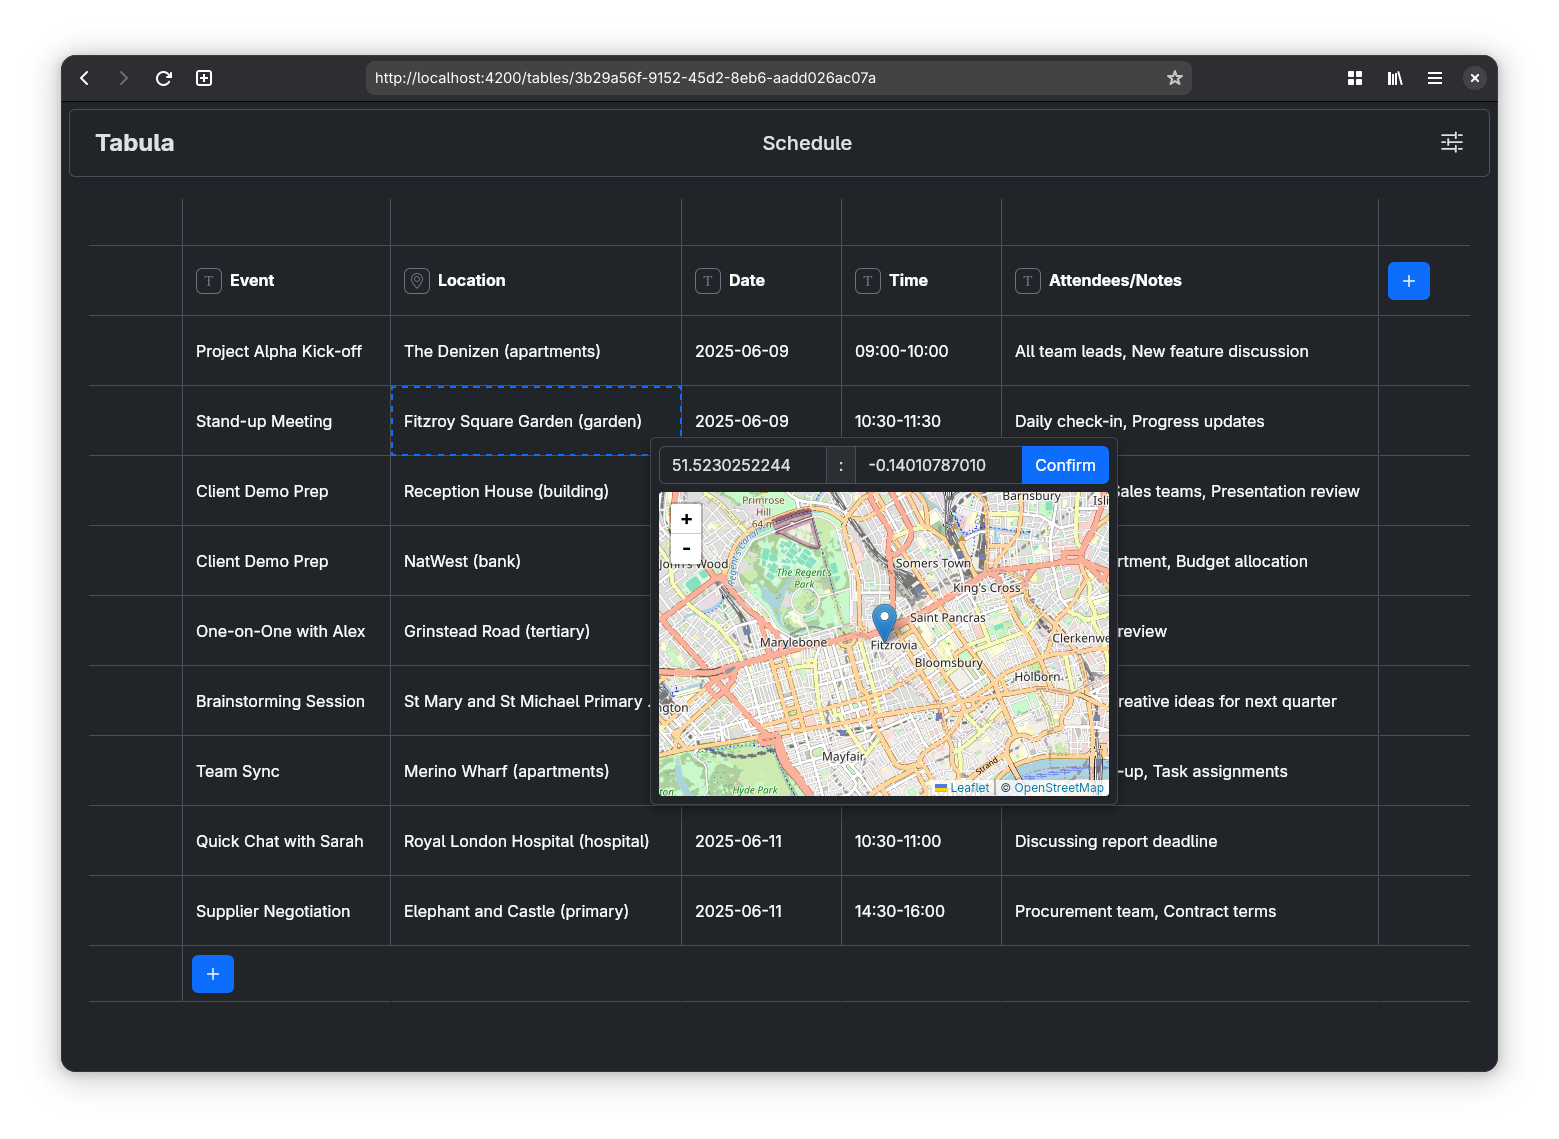
\includegraphics[width=\textwidth]{demo}
  \centering  \href{https://github.com/bytestrick/tabula}{\faGithub\ github.com/bytestrick/tabula}
\end{frame}

\begin{frame}
  \frametitle{Descrizione generale}

  Tabula consente di organizzare dati in formato tabellare facilitando l'accesso e la modifica. Piuttosto che un foglio di calcolo, si può considerare l'app come una base di dati con cui si può interagire direttamente.

  \vspace{10pt}

  Ogni tabella in Tabula è composta da diverse colonne, ognuna con un \textbf{tipo} assegnato: numero, testo, data, posizione geografica, denaro, somma monetaria, ecc.

  \vspace{10pt}

  La facilità di utilizzo delle tabelle le rende uno strumento perfetto per tenere traccia delle letture, sia concluse che pianificate; oppure raggruppare in un unico punto i task pianificati (to-do) e aggregarli in classi usando il tipo \textit{tag}, corredandoli di una data e una posizione geografica opzionalmente; o ancora tracciare la performance di una squadra di calcio, derivando informazioni statistiche dagli esiti delle singole partite.

\end{frame}

\begin{frame}
  \frametitle{Tecnologie usate}

  \begin{itemize}
    \item[\faLeaf] Spring Boot
    \item[\faEnvelope] Spring Email
    \item[\faDatabase] PostgreSQL
  \end{itemize}

  \vspace{15pt}

  \begin{itemize}
    \item[\faHtml5] Angular
    \item[\faCss3] Bootstrap
  \end{itemize}

  \vspace{18pt}

  API esterne:
  \begin{itemize}
    \item[\faMapMarker] \href{https://www.openstreetmap.org/}{OpenStreetMap}
    \item[\faMapSigns] \href{https://nominatim.openstreetmap.org/}{Nominatim}
  \end{itemize}
\end{frame}

\begin{frame}
  \frametitle{Modello entità relazione}
  \begin{figure}
    % \includegraphics[width=\textwidth]{entity_relation_diagram}
    \texttt{TODO: includere modello ER}
  \end{figure}
\end{frame}

\begin{frame}
  \frametitle{Diagramma di classi (back-end)}
  \begin{figure}
    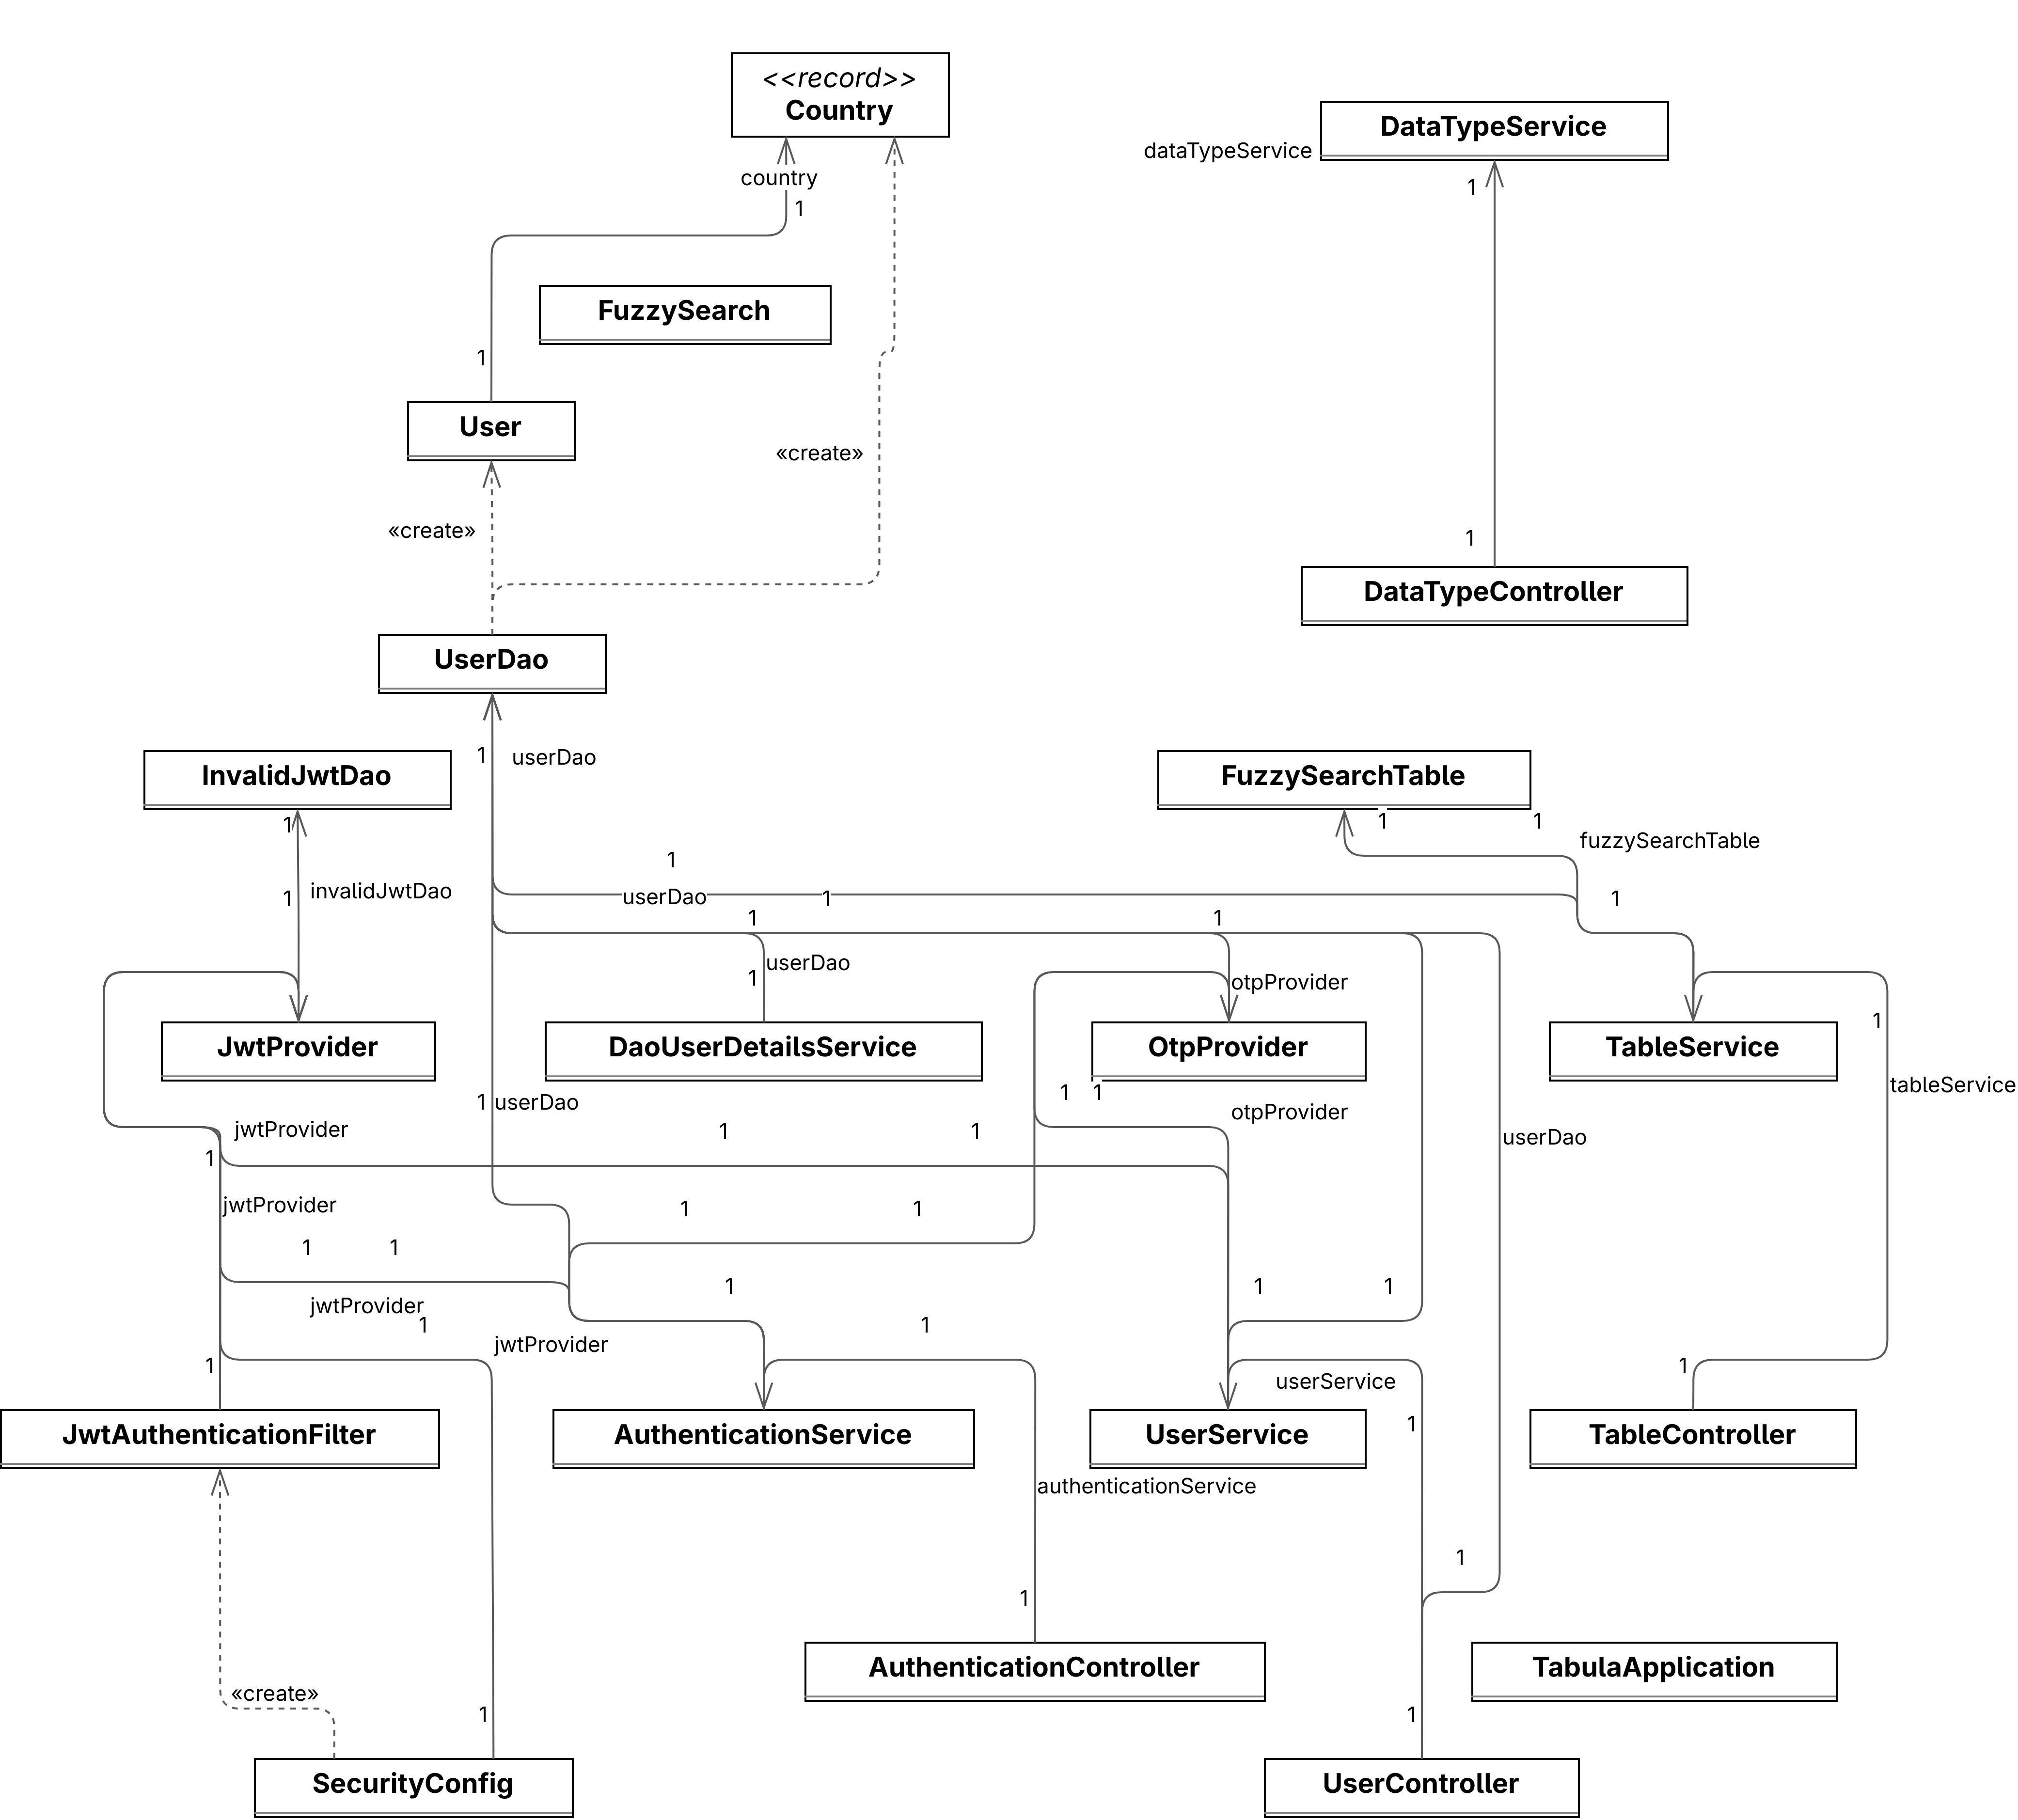
\includegraphics[height=8cm]{classes}
  \end{figure}
\end{frame}

\end{document}
